\section{Computational Implementation}
\subsection[Overview]{Gibbs Energy Minimiser - Overview}

\frame{
	\frametitle{Computational Structure}
	\begin{figure}[htbp]
		\begin{center}
		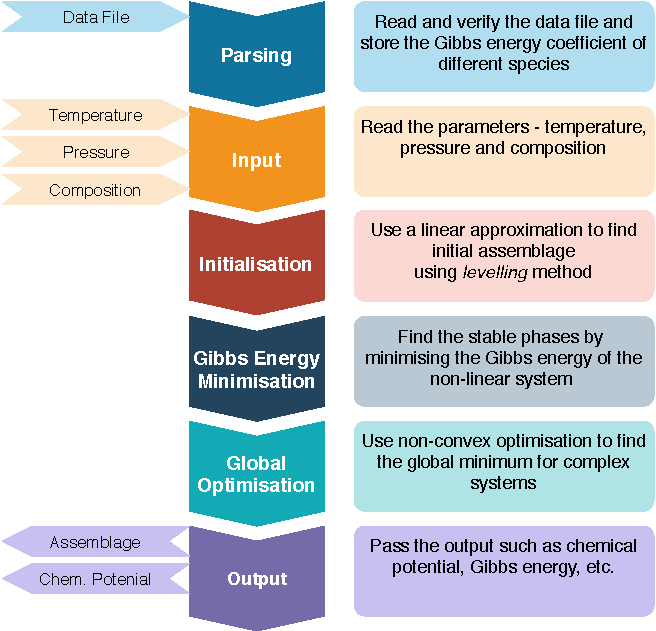
\includegraphics[height=0.65\paperheight]{Figures/YJ_structure.pdf}
		\end{center}
	\end{figure}
}

\subsection{Gibbs Energy Minimiser}
    \frame{
    \frametitle{Parsing and Input}
    
         \only<1>{
             \begin{itemize}
                 \item<1-> The data files are created using the well known Calphad method and can be available in different formats.
             \end{itemize}
             }
         \only<2>{\begin{figure}
                 \centering
                 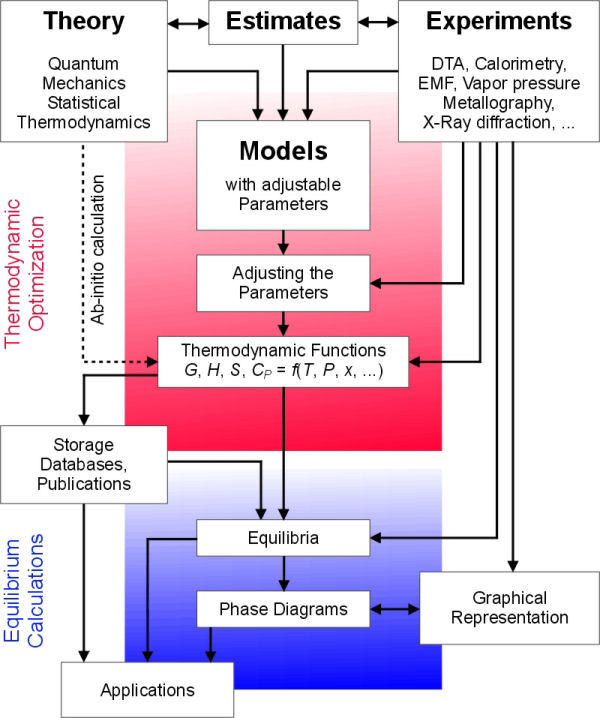
\includegraphics[height=0.75\paperheight]{Figures/Calphad_method.jpg}
             \end{figure}}
         \only<3-4>{
             \begin{itemize}
                 \item<3-> The data files are created using the well known Calphad method and can be available in different formats.
                 \item<3-> Most commonly used formats are ThermoCalc (*.tdb) and ChemSage (*.dat).
                 \item<4-> Yellowjacket uses ChemSage (*.dat) format datafiles, which can be generated by the commercial software FactSage.
                 \item<5-> Temperature, pressure and composition are required at each time step and for each mesh element.
                 \item<6-> At each time step MOOSE can provide these inputs to Yellowjacket.
             \end{itemize}}
  }

    \frame{
    \frametitle{Initialisation}
             \begin{itemize}
                 \item<1-> Gibbs energy minimisers require an initial estimate of molar quantities of species and phases.
                 \item<2-> \textit{Levelling} is an estimating process developed by Eriksson and Thompson (1989).
                 \item<3-> Levelling temporarily converts the non-linear optimisation problem into a linear optimisation problem by treating all species and phases as pure separate phases.
                 \item<4->The number of iterations required to achieve convergence does not increase rapidly with the number of system components.
             \end{itemize}
    }
    
%      \frame{
%    \frametitle{Initialisation}
%         \begin{figure}
%             \centering
%             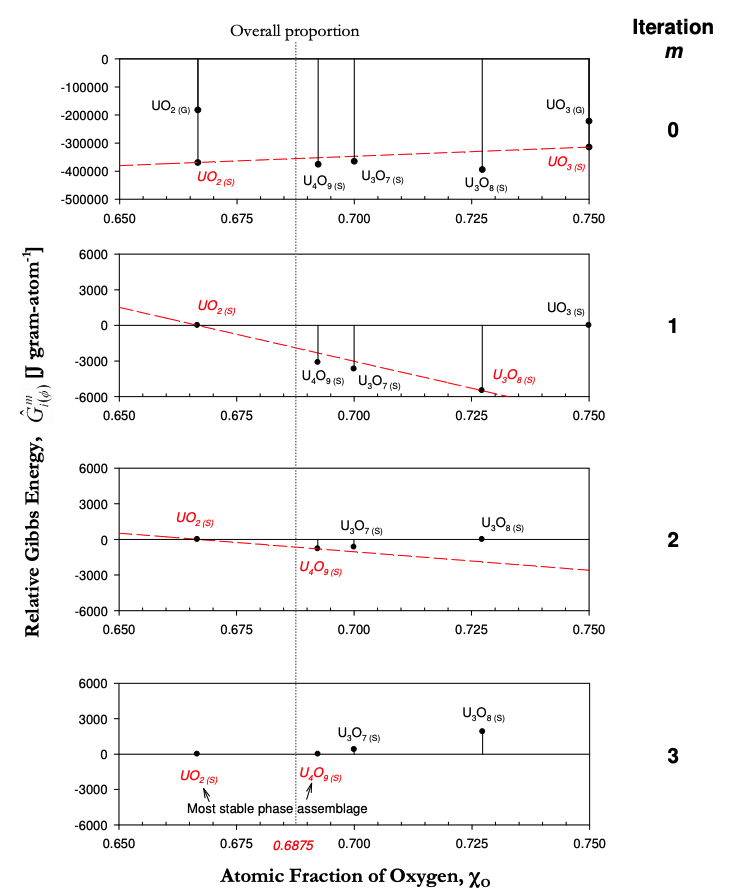
\includegraphics[height=0.75\paperheight]{Figures/Levelling_illustration}
%         \end{figure}
%      }
    
    \frame{
    \frametitle{Initialisation}
     \begin{multicols}{2}
         \begin{itemize}
             \item Initialise using neighbour cells
             \begin{figure}
                 \centering
                 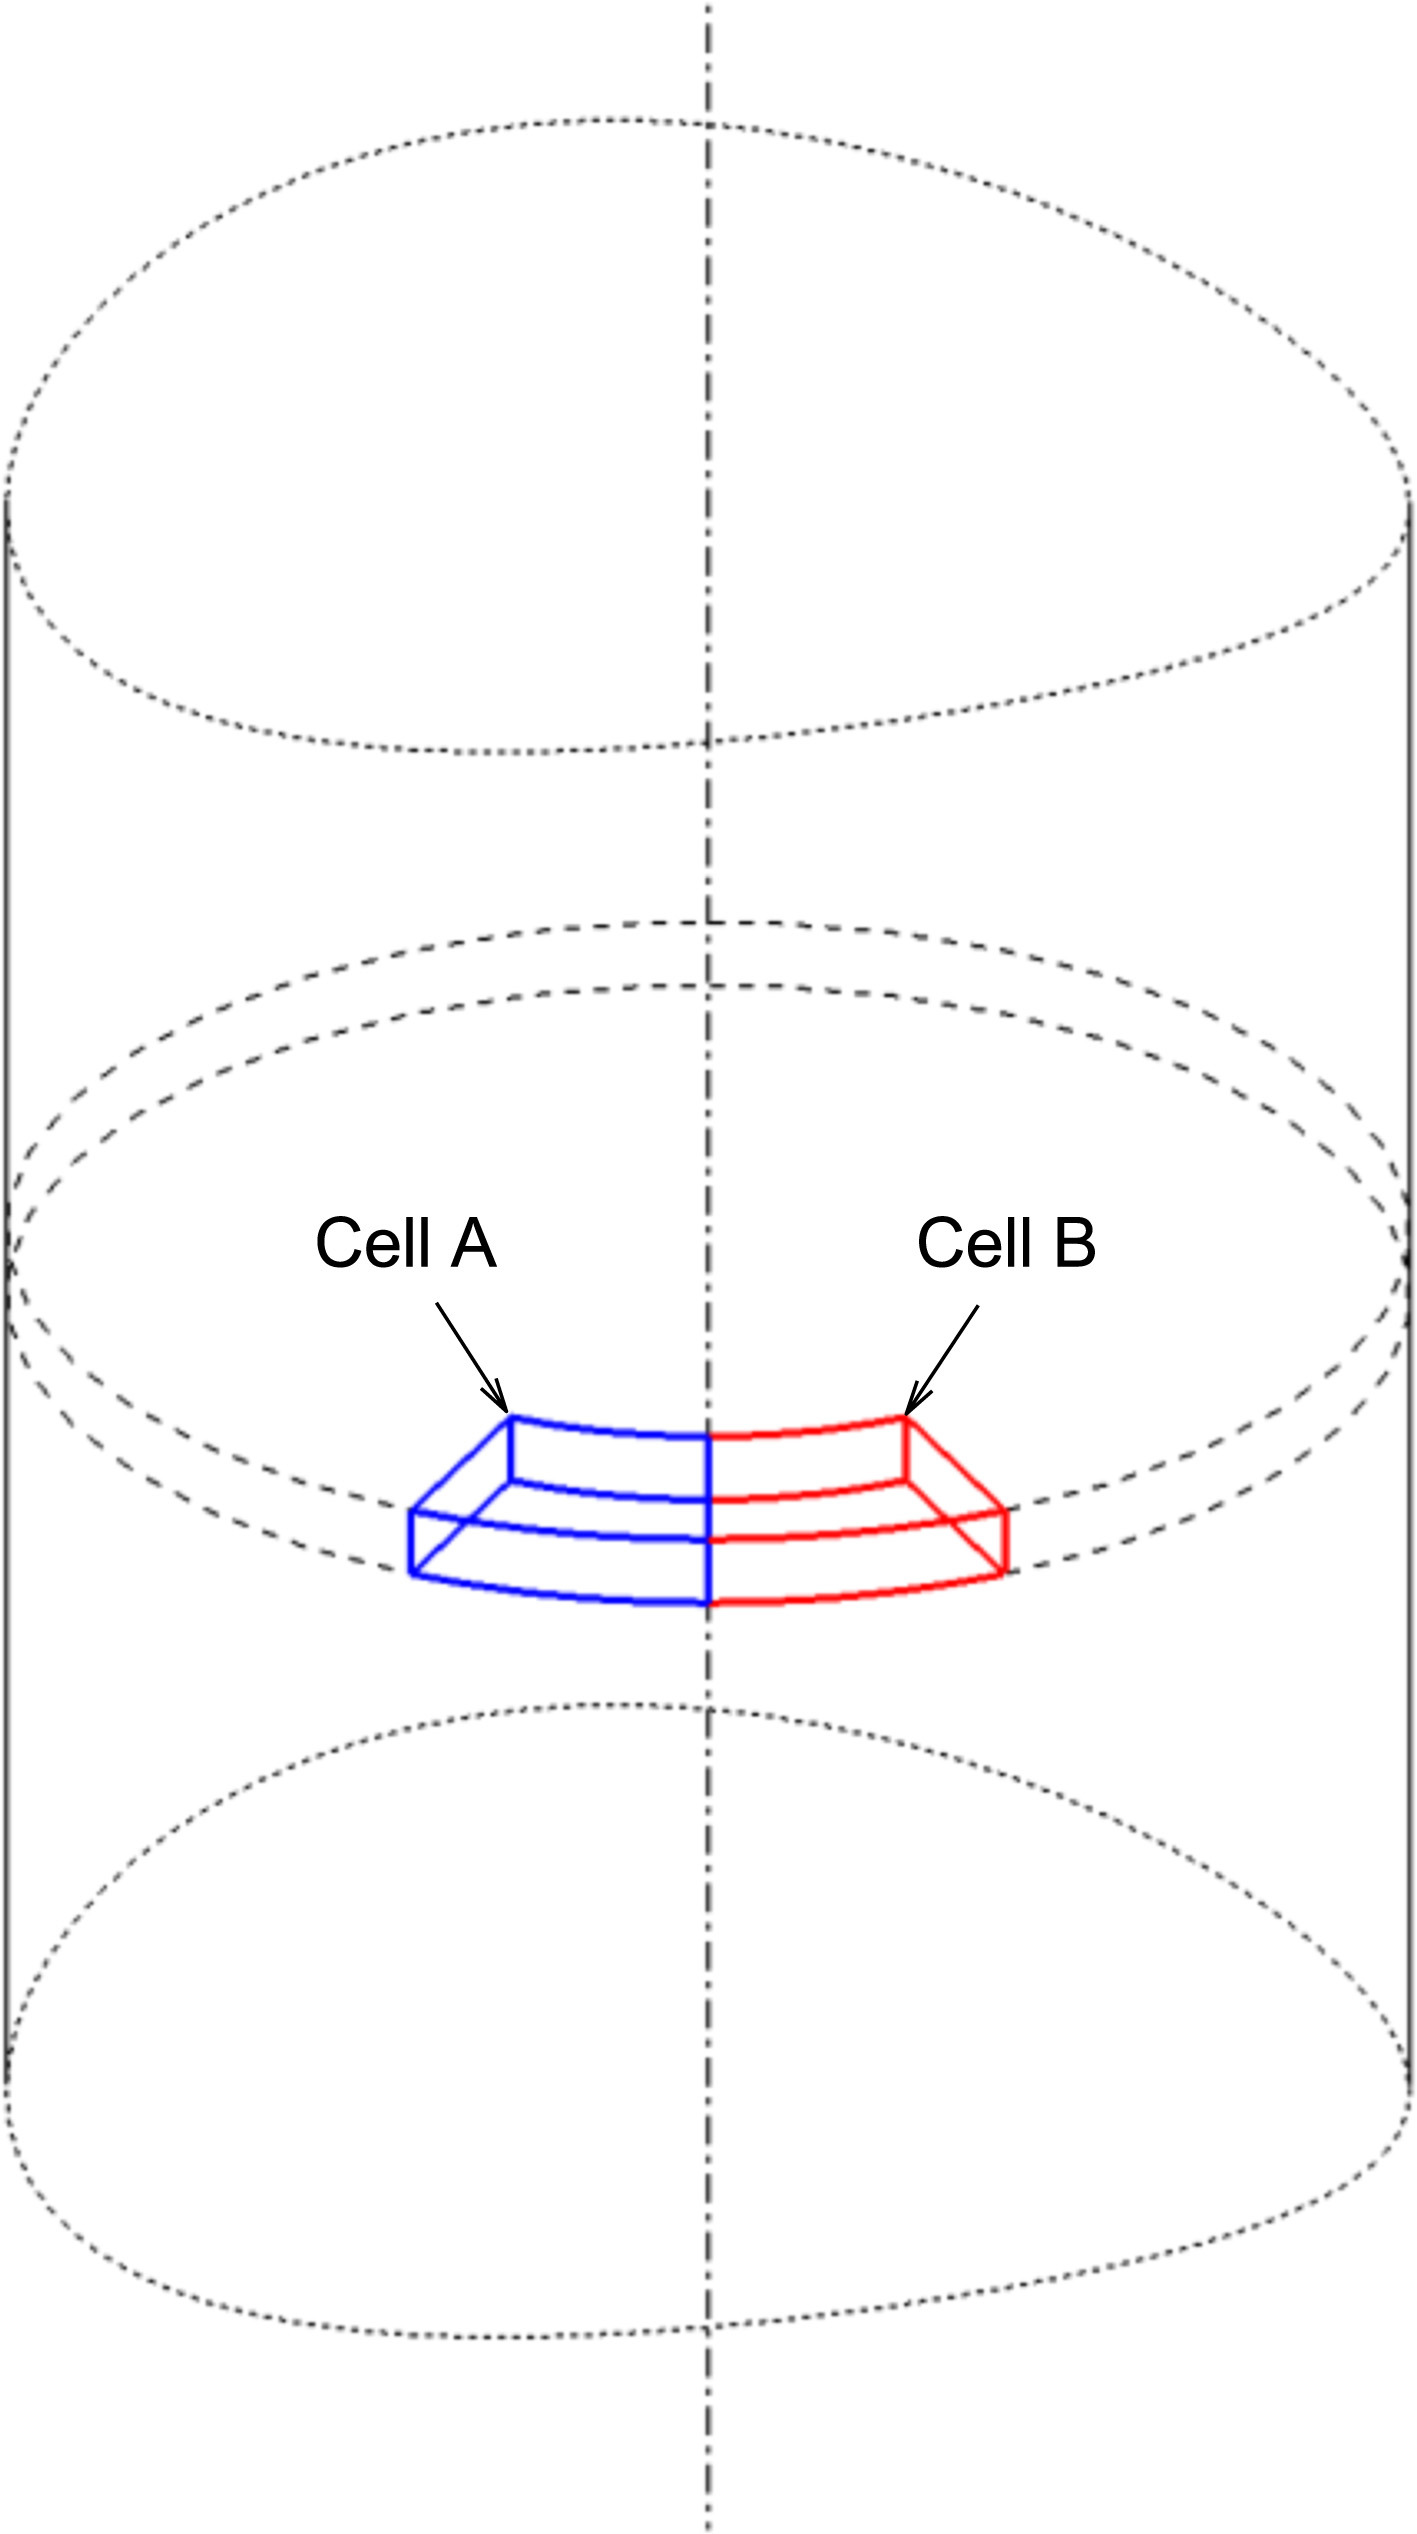
\includegraphics[width=0.575\linewidth]{Figures/rest.jpg}
             \end{figure}
         \end{itemize}
         \columnbreak
         \begin{itemize}
             \item Initialise with last time step
             \begin{figure}
                 \centering
                 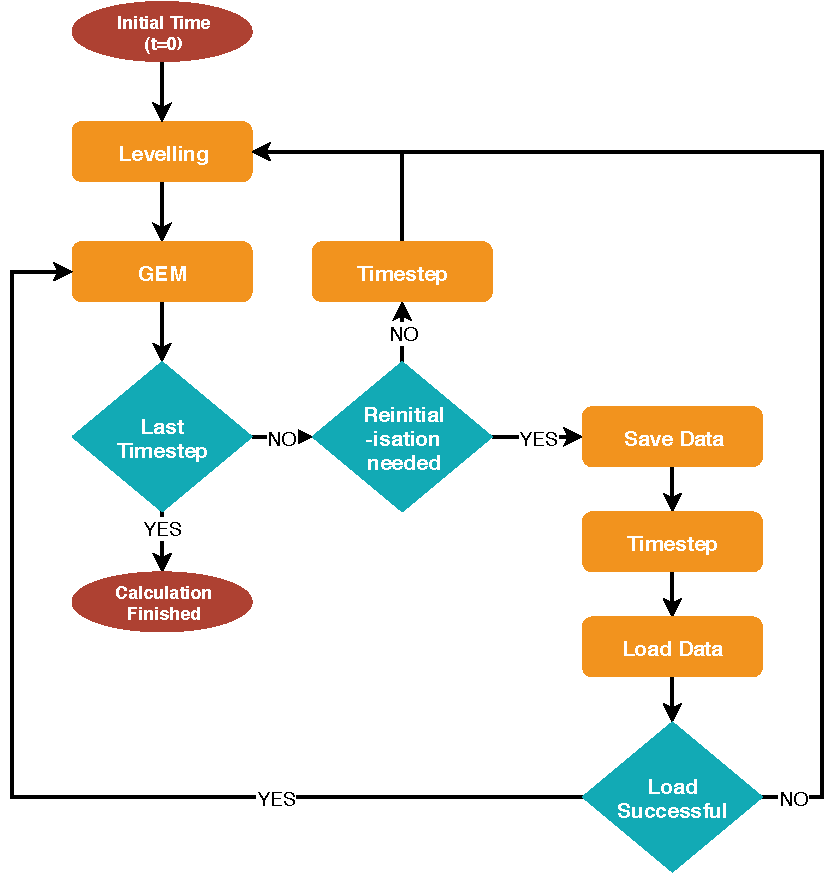
\includegraphics[width=0.925\linewidth]{Figures/Initialisation.pdf}
             \end{figure}
         \end{itemize}
     \end{multicols}
    }

    
     \frame{
     \frametitle{Gibbs Energy Minimisation}
         \onslide<1-4>{\begin{itemize}
 	        \item<1-> GEM uses the method of Lagrange multipliers resulting in the following system of equations \[\mtx{H}\cdot\vec{\pi}=\vec{\zeta}\]
 	    \end{itemize}}
	    \scriptsize
\only<2>{\begin{equation*}\label{eq:Hessian_mat}
        \mathbf{H} = 
        \begin{bmatrix}
            r_{j=1,k=1} & \dots & r_{j=1,k=C} & \phi_{j=1,\lambda=1} & \dots & \phi_{j=1,\lambda=\Lambda} & \nu_{j=1,\omega=1} & \dots & \nu_{j=1,\omega=\Omega} \\
            \vdots & \ddots & \vdots & \vdots & \ddots & \vdots & \vdots & \ddots & \vdots \\
            r_{j=C,k=1} & \dots & r_{j=C,k=C} & \phi_{j=C,\lambda=1} & \dots & \phi_{j=C,\lambda=\Lambda} & \nu_{j=C,\omega=1} & \dots & \nu_{j=C,\omega=\Omega} \\
            \phi_{\lambda=1,j=1} & \dots & \phi_{\lambda=1,j=C} & 0 & \dots & 0 & 0 & \dots & 0 \\
            \vdots & \ddots & \vdots & \vdots & \ddots & \vdots & \vdots & \ddots & \vdots \\
            \phi_{\lambda=\Lambda,j=1} & \dots & \phi_{\lambda=\Lambda,j=C} & 0 & \dots & 0 & 0 & \dots & 0 \\
            \nu_{\omega=1,j=1} & \dots & \nu_{\omega=1,j=C} & 0 & \dots & 0 & 0 & \dots & 0 \\
            \vdots & \ddots & \vdots & \vdots & \ddots & \vdots & \vdots & \ddots & \vdots \\
            \nu_{\omega=\Omega,j=1} & \dots & \nu_{\omega=\Omega,j=C} & 0 & \dots & 0 & 0 & \dots & 0 
        \end{bmatrix}
    \end{equation*}}
    
    \only<3>{ \begin{equation*}\label{eq:LagMult_mat}
        \boldsymbol{\pi} = 
        \begin{bmatrix}
            \pi_{j=1}^{m+1} \\
            \vdots \\
            \pi_{j=E}^{m+1} \\
            \pi_{\lambda=1}^{m+1} \\
            \vdots \\
            \pi_{\lambda=\Lambda}^{m+1} \\
            \pi_{\omega=1}^{m+1} \\
            \vdots\\
            \pi_{\omega=\Omega}^{m+1}
        \end{bmatrix}
    \end{equation*}}
    
    \only<4>{ \begin{equation*}\label{eq:Constraint_mat}
        \boldsymbol{\zeta} = 
        \begin{bmatrix}
            b_{j=1} +  \sum_{\lambda=1}^{\Lambda} \sum_{i=1}^{N_\lambda} \left( \frac{\mu_{i(\lambda)}^{m}}{RT} -1 \right)n_{i(\lambda)}^{m} \nu_{i,j=1}\\
            \vdots \\
            b_{j=E} +  \sum_{\lambda=1}^{\Lambda} \sum_{i=1}^{N_\lambda} \left( \frac{\mu_{i(\lambda)}^{m}}{RT} -1 \right)n_{i(\lambda)}^{m} \nu_{i,j=E}\\
            \sum_{i=1}^{N_{\lambda=1}} \left( \frac{\mu_{i(\lambda=1)}^{m}}{RT} -1 \right)n_{i(\lambda=1)}^{m} \\
            \vdots \\
            \sum_{i=1}^{N_{\lambda=\Lambda}} \left( \frac{\mu_{i(\lambda=\Lambda)}^{m}}{RT} -1 \right)n_{i(\lambda=\Lambda)}^{m} \\
            \frac{\mu_{\omega=1}^{m}}{RT} \\
            \vdots\\
            \frac{\mu_{\omega=\Omega}^{m}}{RT} \\
        \end{bmatrix}
    \end{equation*}
}
    }
    
%     \begin{frame}{Gibbs Energy Minimisation}
%         \begin{itemize}
% 	        \item Phase assemblage algorithm
% 	    \end{itemize}
% 	    \begin{figure}
% 	        \centering
% 	        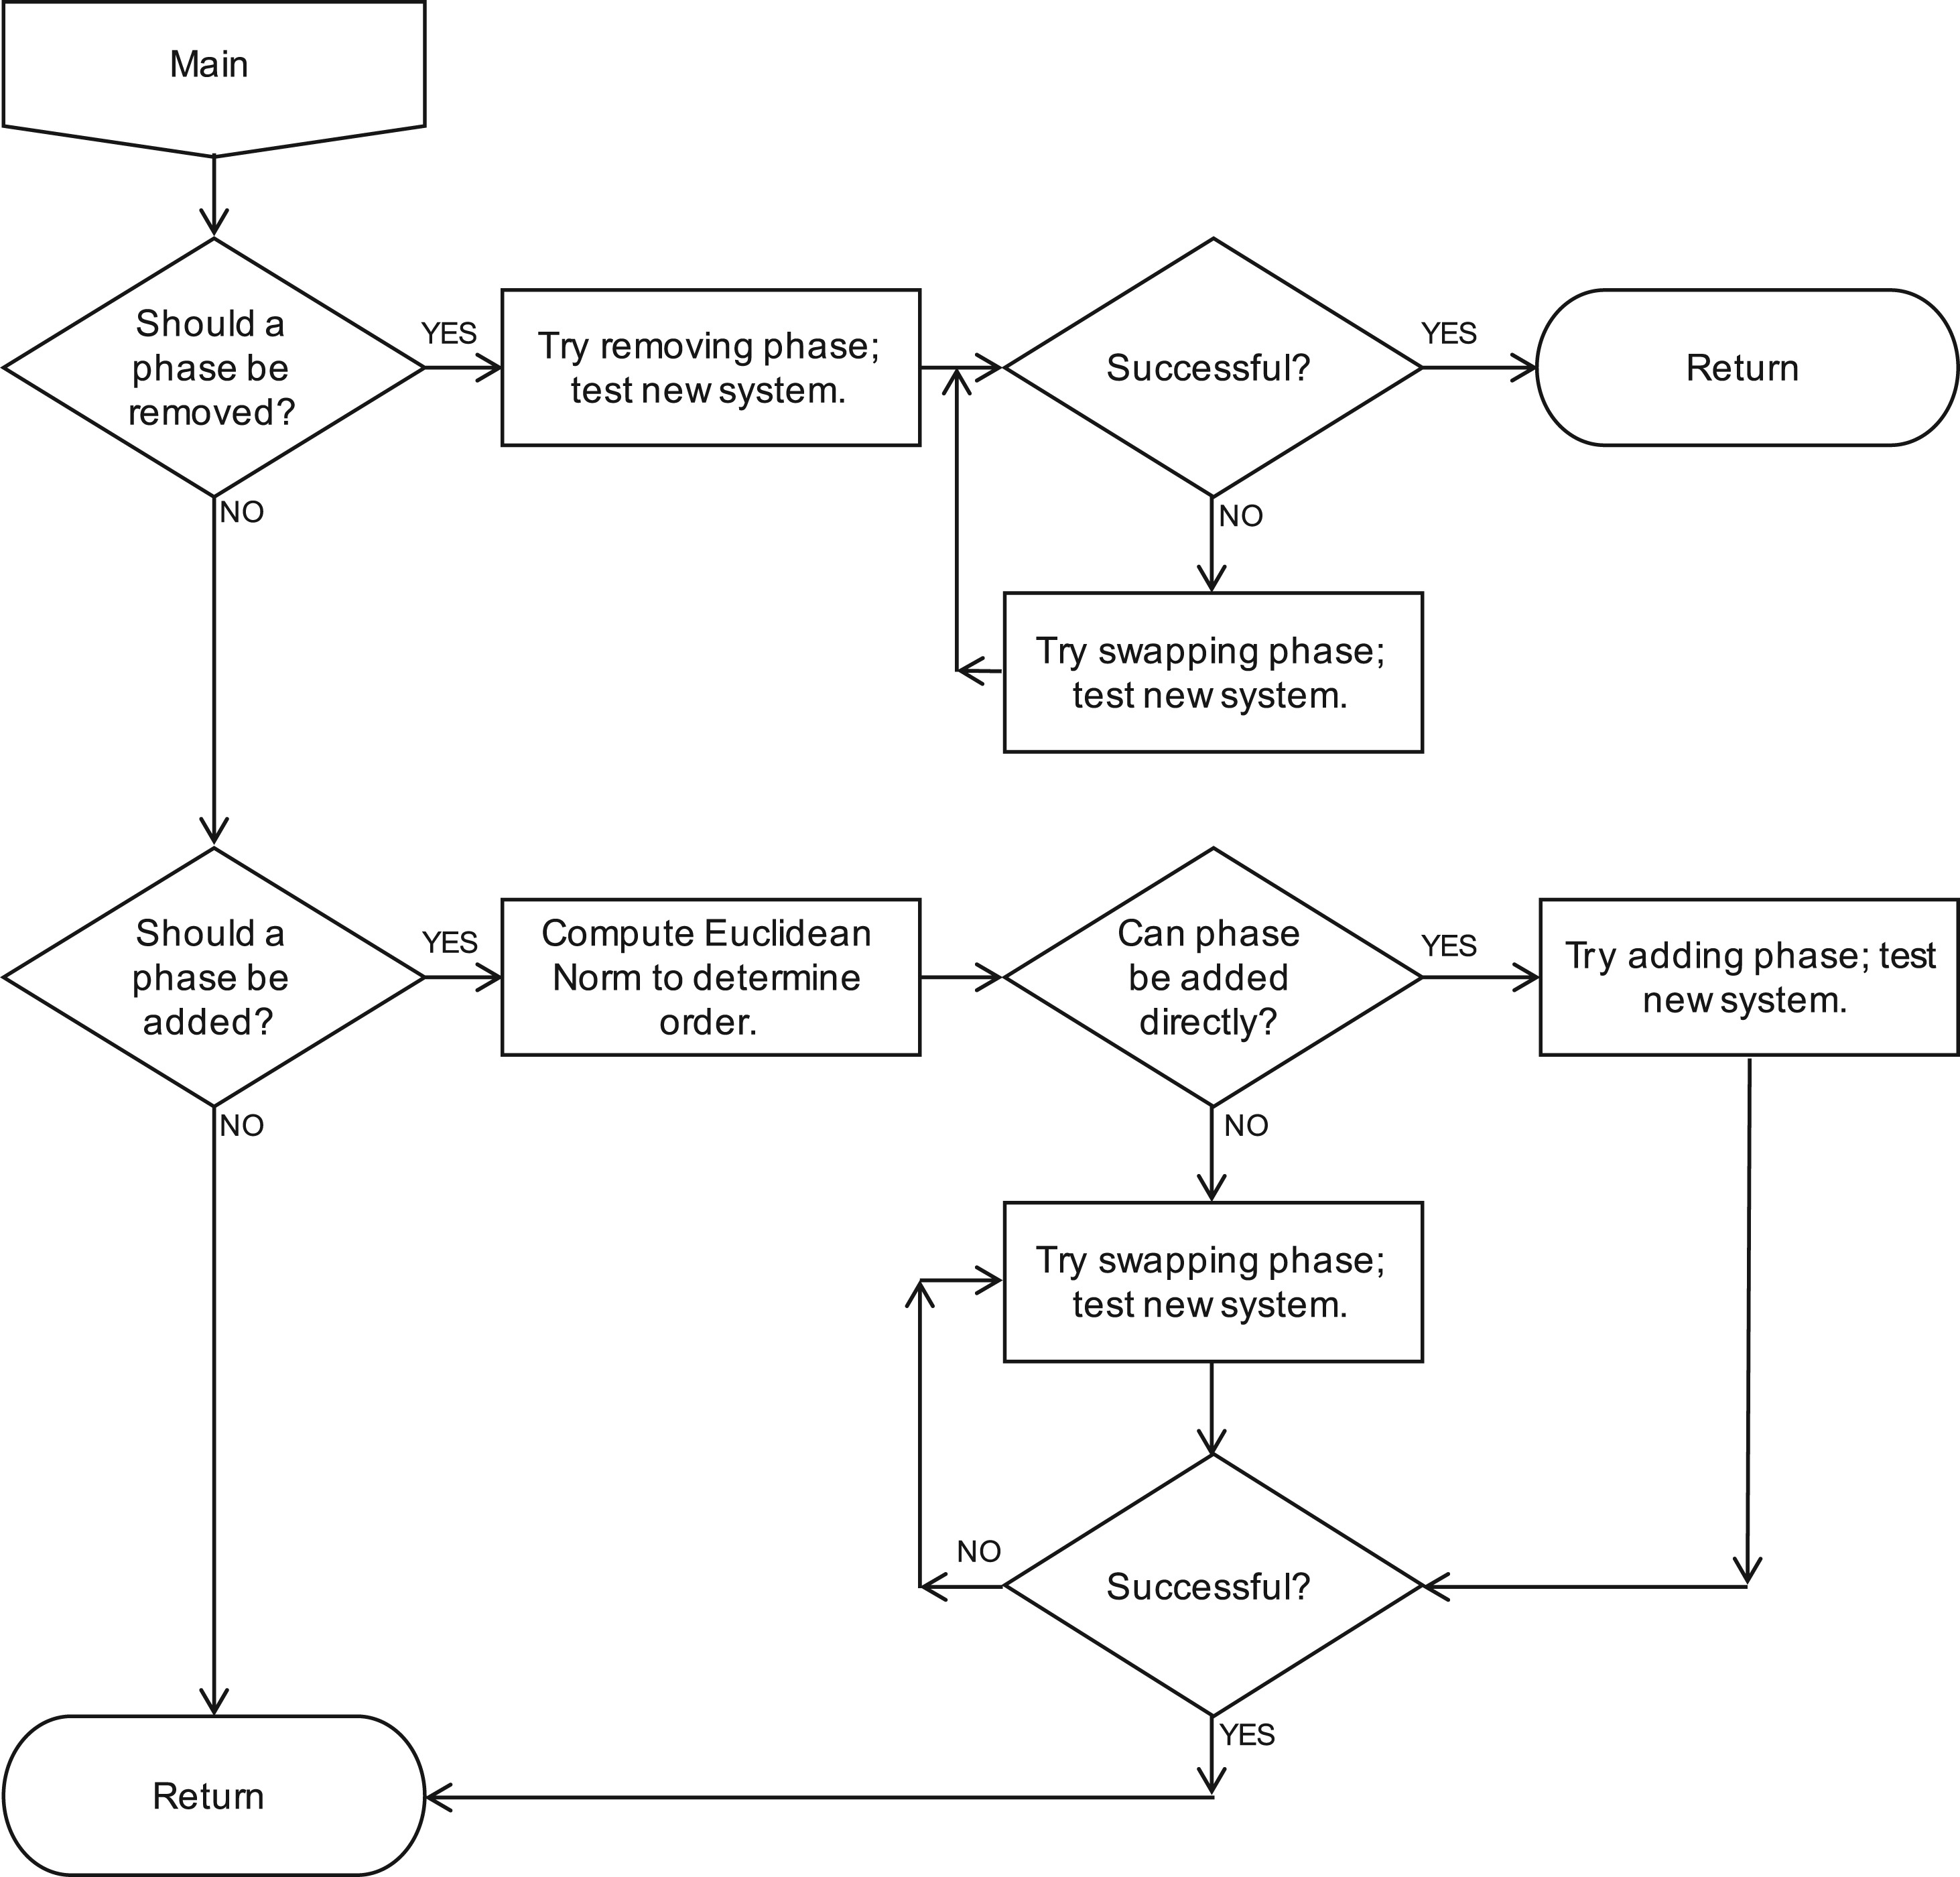
\includegraphics[width=0.45\linewidth]{Figures/Phase_assemblage.jpg}
% 	    \end{figure}
%     \end{frame}
%    
%     \begin{frame}{Gibbs Energy Minimisation}
%         \begin{itemize}
% 	        \item Line Search algorithms
% 	   % \end{itemize}
% 	    \begin{figure}
% 	        \centering
% 	        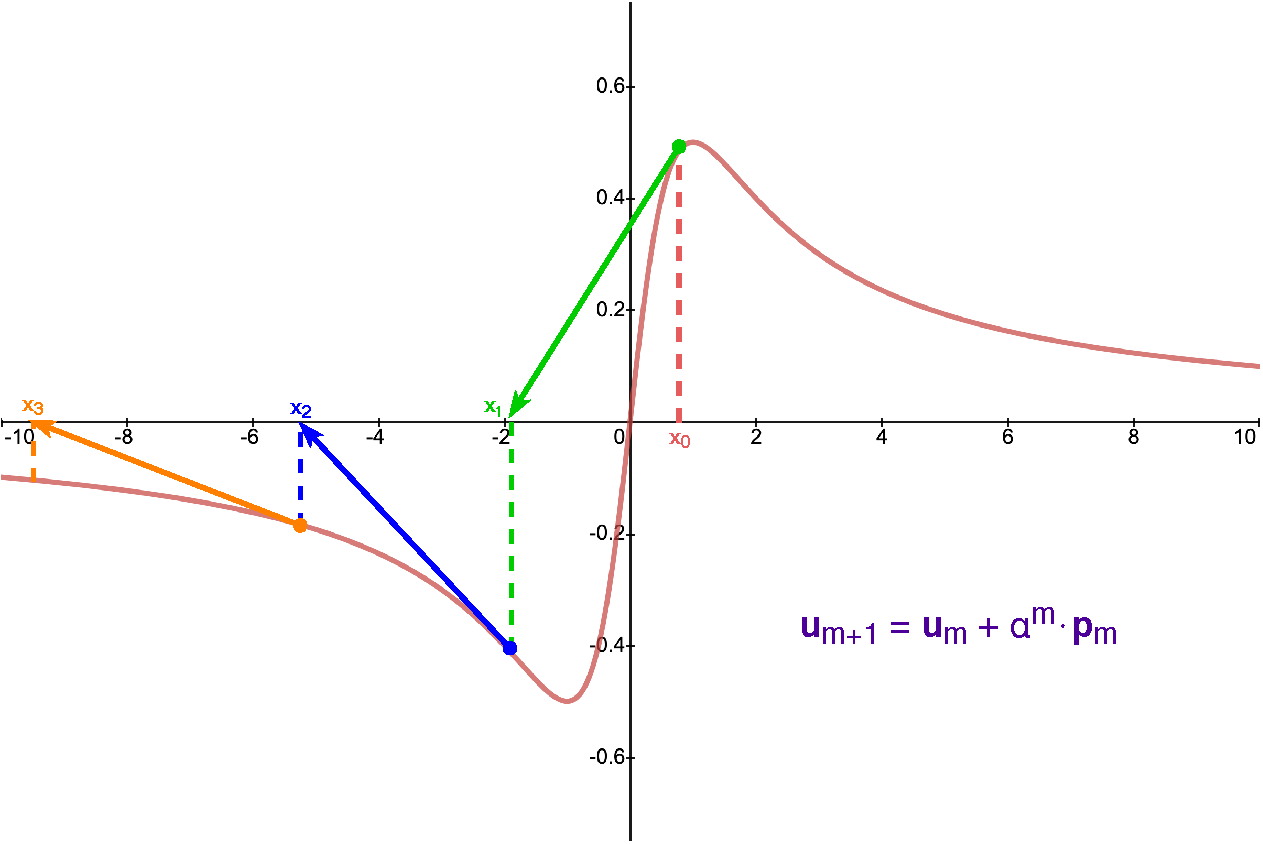
\includegraphics[width=0.5\paperwidth]{Figures/Line_search.pdf}
% 	    \end{figure}
% 	   % \begin{itemize}
% 	        \item Use of Wolfe/Armijo conditions can help avoid divergence.
% 	    \end{itemize}
%     \end{frame}
    
     \begin{frame}{Global Optimisation}
         \begin{itemize}
             \item The Gibbs energy function of non-ideal phases may be non-convex, yielding multiple local minima. This makes finding global minimum a challenge.
         \end{itemize}
         \begin{figure}
             \centering
             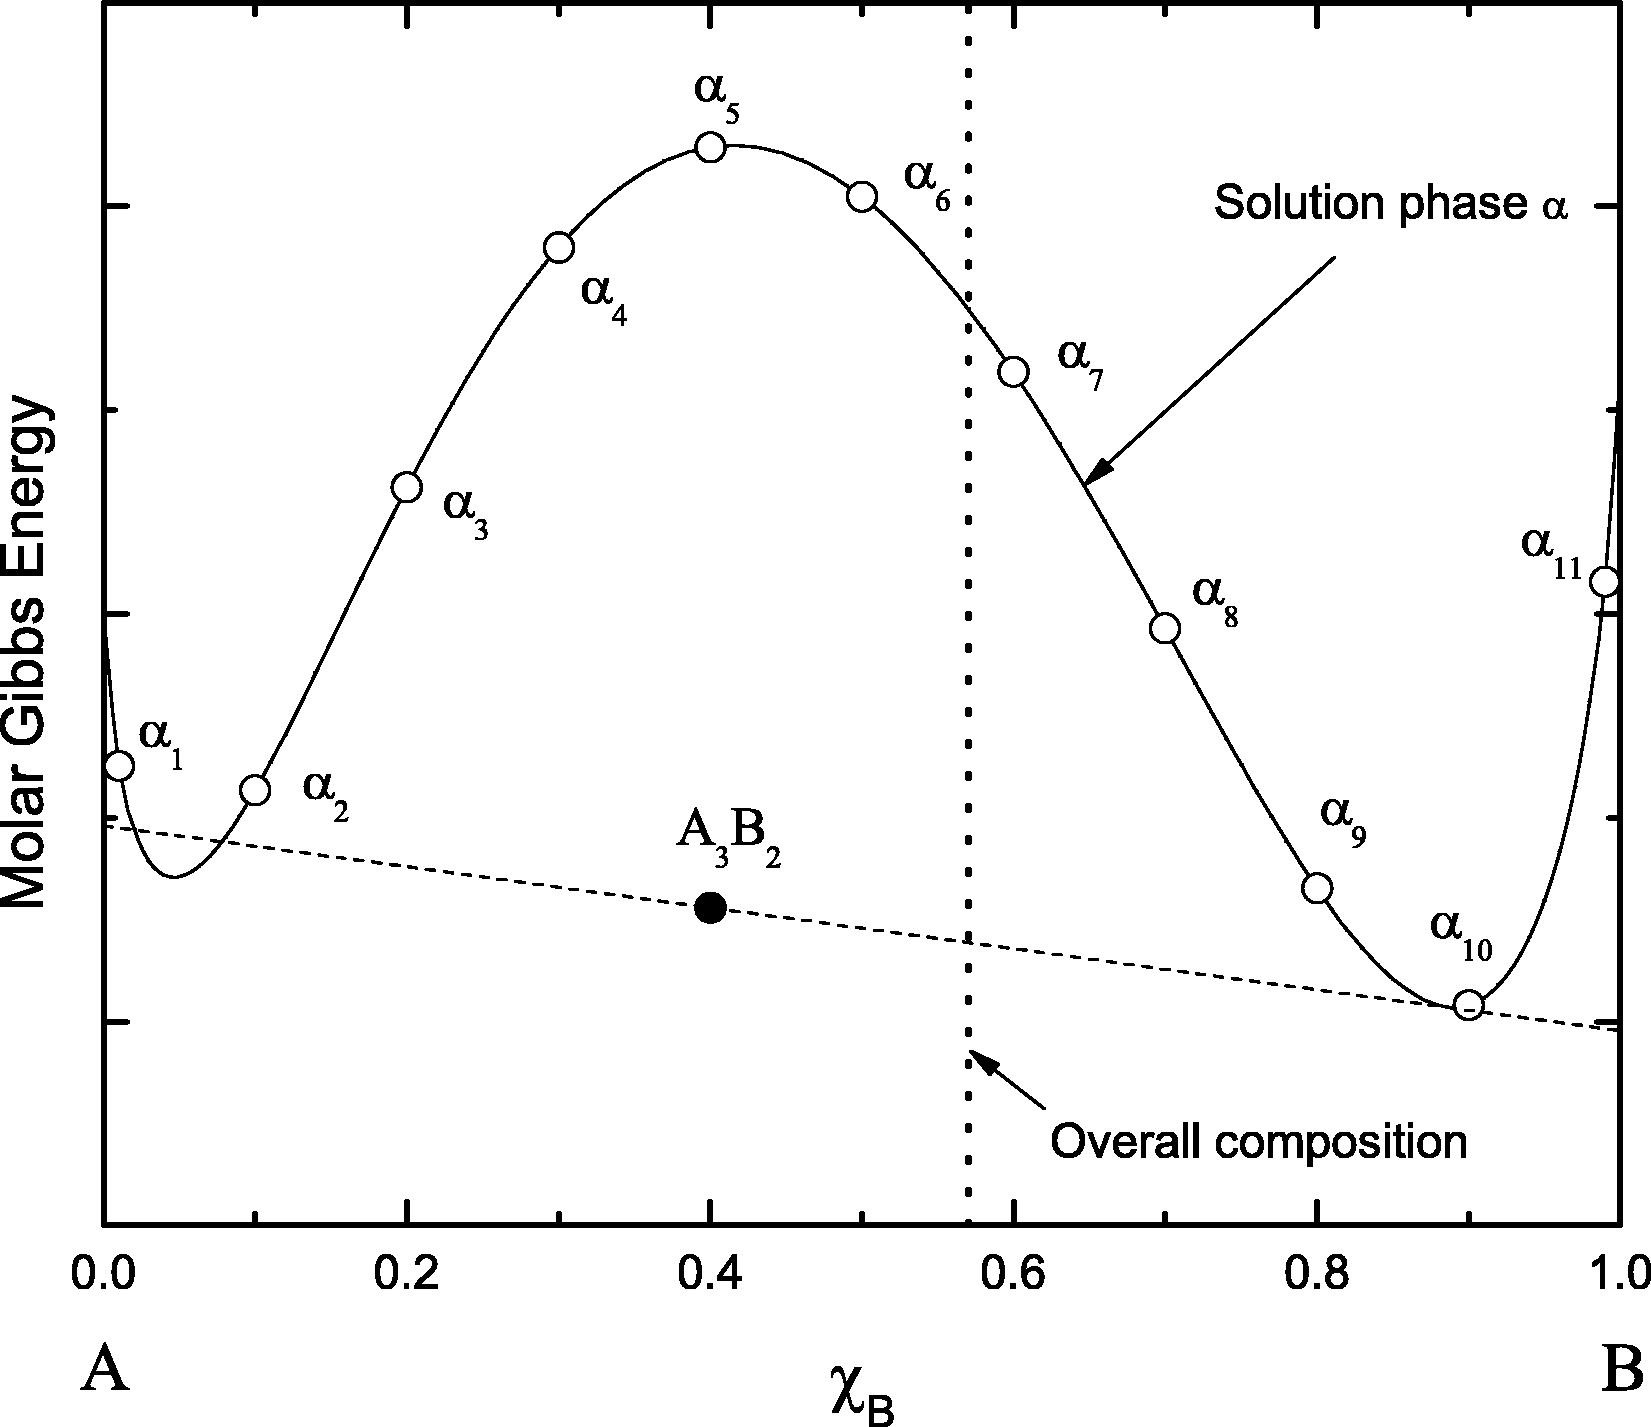
\includegraphics[width=0.5\linewidth]{Figures/Global_opt1}
         \end{figure}
     \end{frame}
    

     \begin{frame}{Output}
         \begin{itemize}
             \item Outputs after the Gibbs energy minimisation and global optimisation include moles of phases, species mole fraction in each phase, chemical potentials, Gibbs energy, etc.
             \item The chemical potential of various species can be used to find the driving force for other reactions such as corrosion.
             \item These parameters can also be passed to other MOOSE based codes such as {Marmot} and {Bison}.
         \end{itemize}
     \end{frame}
     
     \subsection{Challenges and Thrust Areas}
     \frame{
     	\frametitle{Challenges and Thrust Areas}
	\begin{itemize}
		\item<+-> Initialisation
			\begin{itemize}
				\item<+-> Levelling + GEM can often be costly in multiphysics simulations.
				\item<+-> Principles of continuum can be used to reduce the computational time.
				\item<+-> Using solution from previous time step as initial estimate. For example,  Thermochimica - Bison coupled problems have been accelerated by up to 7X.
				\item<+-> Assemblage from a neighbouring element can potentially be used as an initialisation method.	
			\end{itemize}
		\item<+-> Gibbs Energy Minimisation
			\begin{itemize}
				\item<+-> There is a need to constantly update the phases present in the assemblage - phases might have to be removed, added or exchanged.
				\item<+-> Phase selection algorithm can reduce cycling.
				\item<+-> Line search methods can significantly affect the rate of convergence of Newton solver.
				\item<+-> Armijo/Wolfe conditions must be efficiently implemented to make sure that Newton steps do not lead to divergence.
			\end{itemize}
	\end{itemize}
     }
     
     \frame{
     	\frametitle{Challenges and Thrust Areas}
	\only<1-5>{
	\begin{itemize}
		\item<+-> Global Optimisation
			\begin{itemize}
				\item<+-> Mathematically, global optimisation implies finding the Gibbs plane that satisfies the sufficient condition: \[\pi_{\lambda} = \min_{\lambda} \sum_{i=1}^{N_{\lambda}}x_{i({\lambda})} \left (\mu_{i({\lambda})} - \sum_{j=1}^C \nu_{i,j}\Gamma_j \right )\]
            			\item<+-> No global optimisation technique guarantees the ability of finding a global extremum of a non-convex function.
             			\item<+-> Searching for a global minimum becomes increasingly more difficult as the size of the system increases.
             			\item<+-> The computational effort associated with performing this task can increase very rapidly in large systems.
			\end{itemize}
	\end{itemize}}
	\only<6-7>{
			\begin{itemize}
				\item<6-> Most commercial codes do not specify the global optimisation method used.
				\item<7-> Originally, they relied on the grid construction method which is a brute force method.
				\begin{figure}
            				\centering
            				 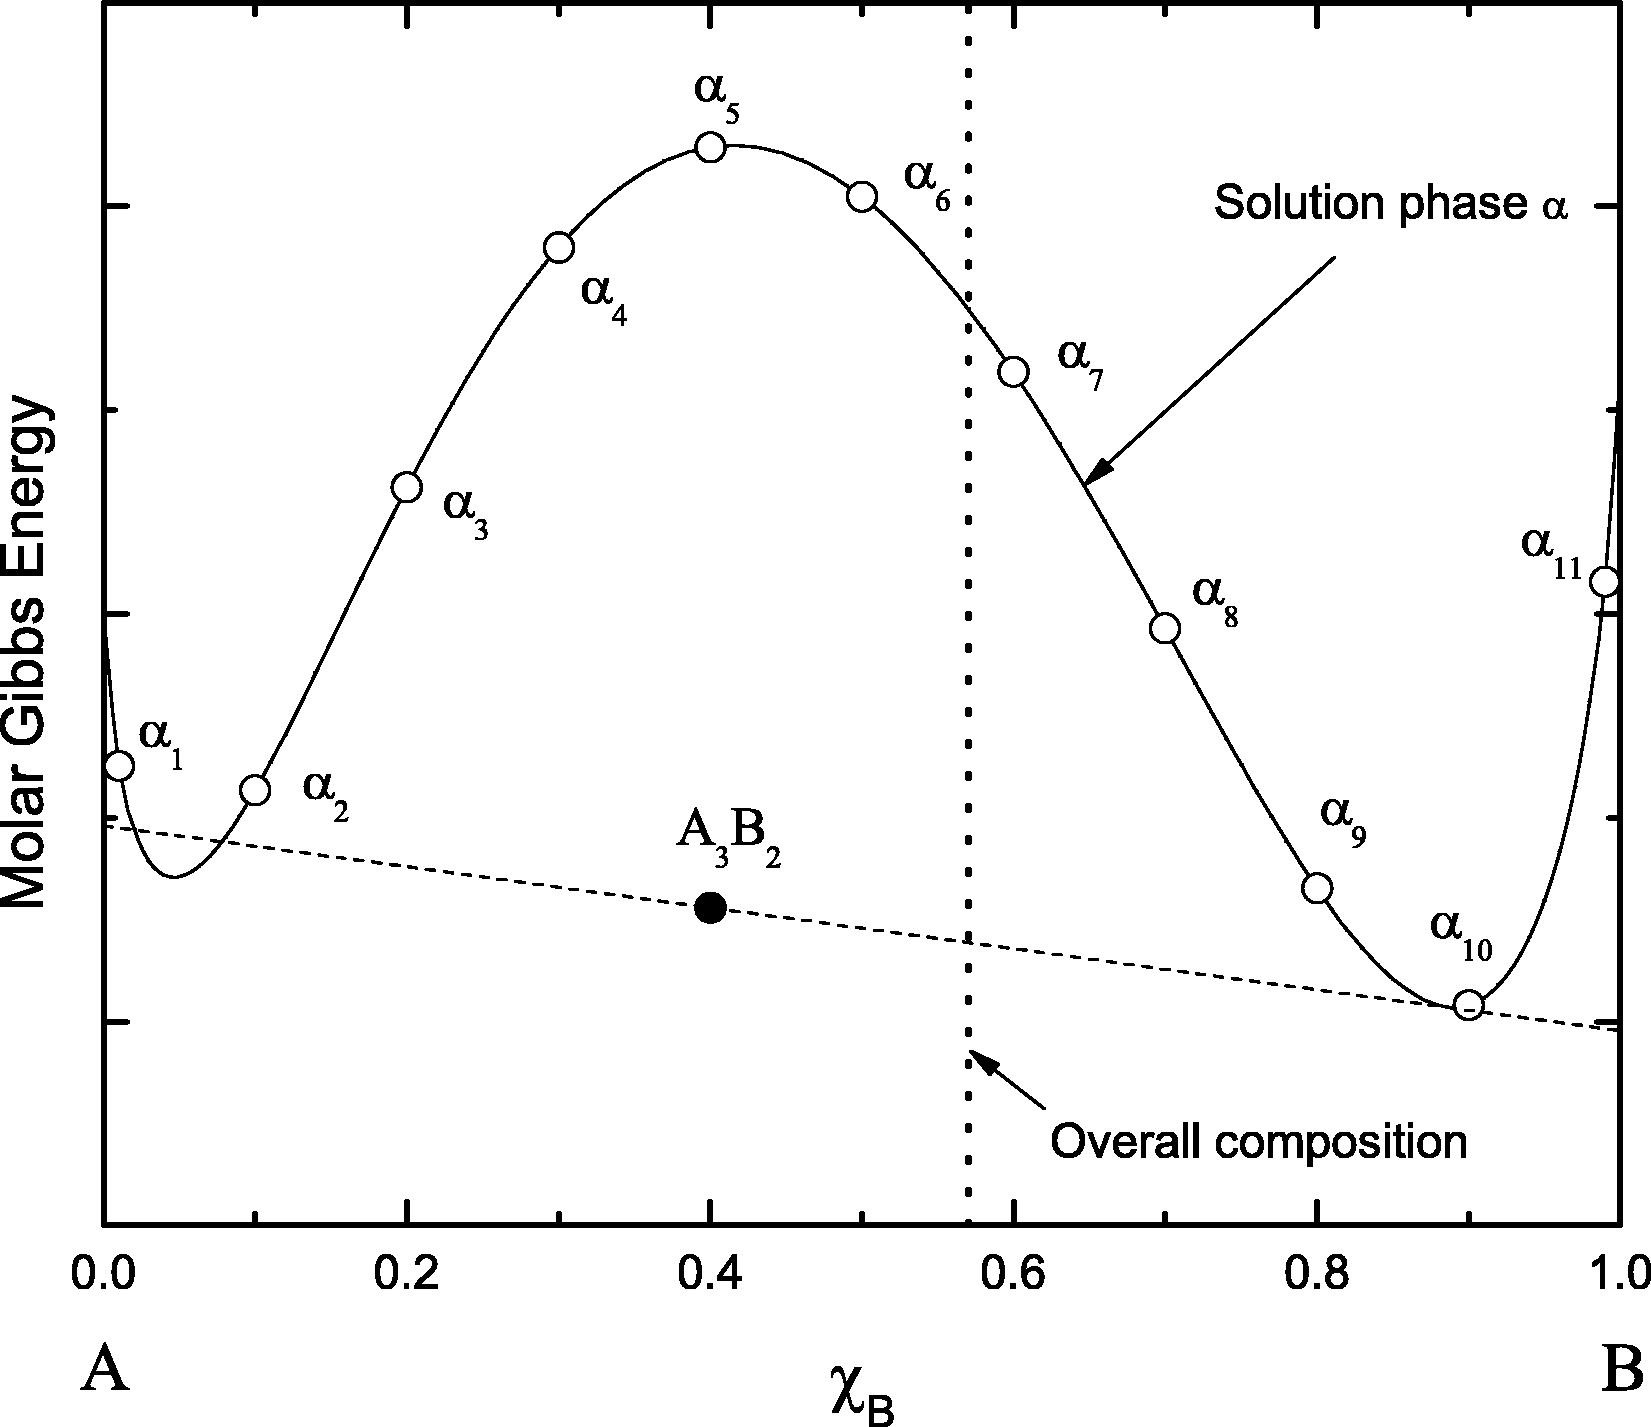
\includegraphics[width=0.55\linewidth]{Figures/Global_opt1}
         			\end{figure}
			\end{itemize}}
	\only<8-9>{
		\begin{itemize}
				\item<+-> Use the advanced algorithms available in literature to improve global optimisation for the thermochemistry solver.
				\item<+-> Through numerical experiments, perform a comprehensive review of both deterministic and stochastic methods of global optimisation applied to computational thermodynamics.
				\item<+-> implement the most suitable optimisation scheme.
			\end{itemize}}
     }
     
     
     \frame{
     	\frametitle{Challenges and Thrust Areas}
	\begin{itemize}
		\item<+-> Coupling to Phase Field method
			\begin{itemize}
				\item<+-> Coupling can result in a very large number of calls between the two modules.
				\item<+->	Potential use of a database of solutions.
				\item<+-> Interpolation of values between different solves.
			\end{itemize}
		\item<+-> Software Quality Assurance
			\begin{itemize}
				\item<+-> Use of CIVET for continuous testing and integration.
				\item<+-> A test suite will be developed for verification.
				\item<+-> Rigorous documentation of every function and their dependencies.
			\end{itemize}
	\end{itemize}
     }
     
     
     
     
     
     
     
     
     
     